\Exercise[number={4}]
A variable \(x\) in \(\mathbf{R}^2\) is emitted by two possible sources,
\(w_1\) and \(w_2\), of probability \(Pr(w_1)=p\) and \(Pr(w_2)=1-p\). 
We want to design a Bayes classifier that assigns the correct class to each
observed \(x\). If the \(p(x|w_i)\) both have a Gaussian distribution, with
mean \(\mu_i\) and variance \(I\sigma_i^2\) (with \(\sigma_1>\sigma_2\)),
draw boundaries of the decision regions for \(p=0.5\).
What happens to these contours if \(p>0.5\) or \(p<0.5\)?

\Answer[number={4}]
The decision boundaries of a binary classifier can be studied by computing the
sign of \(z(x)\), with \(z\) being the exponent of the sigmoid function, in
particular the decision boundaries are given by \(z(x)=0\).
\begin{align*}
    z(x)
    &=\log{\frac{p(x|w_1)}{p(x|w_2)}} + \log{\frac{Pr(w_1)}{Pr(w_2)}}
    =\log{p(x|w_1)}-\log{p(x|w_2)}+\log{\frac{p}{1-p}}\\
    &=-\cancel{\log{\frac{2\pi}{2\pi}}}-\frac{1}{2}\log{\frac{|\Sigma_1|}{|\Sigma_2|}}-\frac{1}{2}(x-\mu_1)^T\Sigma_1^{-1}(x-\mu_1)+\frac{1}{2}(x-\mu_2)^T\Sigma_2^{-1}(x-\mu_2)+\log{\frac{p}{1-p}}\\
    &=-\frac{1}{2\sigma_1^2}(x-\mu_1)^T(x-\mu_1)+\frac{1}{2\sigma_2^2}(x-\mu_2)^T(x-\mu_2)-\frac{1}{2}\log{\biggl(\frac{\sigma_1^2}{\sigma_2^2}\biggr)^2}+\log{\frac{p}{1-p}}
\end{align*}
Remember that \(|\Sigma_i|=|I\sigma_i^2|=\prod{diag}=(\sigma_i^2)^2\).
\begin{align*}
    z(x)=0
    \Longleftrightarrow
    -\frac{1}{\cancel{2}\sigma_1^2}(x-\mu_1)^T(x-\mu_1)+\frac{1}{\cancel{2}\sigma_2^2}(x-\mu_2)^T(x-\mu_2)-\cancel{\frac{1}{2}}\log{\biggl(\frac{\sigma_1^2}{\sigma_2^2}\biggr)^2}+2\log{\frac{p}{1-p}}=0
\end{align*}
Therefore,
\begin{align*}
    &\Rightarrow
    -\frac{1}{\sigma_1^2}(x^Tx+\mu_1^T\mu_1-2\mu_1^Tx)+\frac{1}{\sigma_2^2}(x^Tx+\mu_2^T\mu_2-2\mu_2^Tx)-\log{\biggl(\frac{\sigma_1^2}{\sigma_2^2}\biggr)^2}+2\log{\frac{p}{1-p}}=0\\
    &\Rightarrow
    \biggl(\frac{1}{\sigma_2^2}-\frac{1}{\sigma_1^2}\biggr)x^Tx-2\biggl(\frac{\mu_2^T}{\sigma_2^2}-\frac{\mu_1^T}{\sigma_1^2}\biggr)x-\frac{\mu_1^T\mu_1}{\sigma_1^2}+\frac{\mu_2^T\mu_2}{\sigma_2^2}-2\log{\frac{\sigma_1^2}{\sigma_2^2}}+2\log{\frac{p}{1-p}}=0
\end{align*}
The various coefficients can be replaced as follow:
\begin{align*}
    \Rightarrow
    ax^Tx-2b^Tx-c=0
    \Rightarrow
    x^Tx-2\frac{b^T}{a}x-\frac{c}{a}=0
    \quad\text{and again}\quad
    x^Tx-2b^{*T}x-c^*=0
\end{align*}
Notice that \(b^T\) and \(b^{*T}\) are vectors, while \(a\), \(c\), and \(c^*\)
are scalar quantities. At this point let's rearrange the equation:
\begin{align*}
    \Rightarrow
    x^Tx-2b^{*T}x-c^*+b^{*T}b^*-b^{*T}b^*=0
    \Rightarrow
    (x-b^*)^T(x-b^*)=c^*+b^{*T}b^*
\end{align*}
The \((x-b^*)\) vector represents a distance between \(x\) and a specific point \(b^*\)
and its square is set equal to a constant value, therefore a circle is actually
obtained as decision boundaries. The center of this circle is
\(
    b^*=\frac{b^T}{a}
    =\frac{\frac{\mu_2^T}{\sigma_2^2}-\frac{\mu_1^T}{\sigma_1^2}}{\frac{1}{\sigma_2^2}-\frac{1}{\sigma_1^2}}
    =\frac{\sigma_1^2\mu_2^T-\sigma_2^2\mu_1^T}{\sigma_1^2-\sigma_2^2}
\)
, while
the circle radius is given by \(\sqrt{c^*+b^{*T}b^*}\).\\
By assuming \(\sigma_1>\sigma_2\), the area inside the decision boundaries enclose
the area for which \(x\) is considered belonging to class \(w_2\), while the area
outside the circle classify \(x\) as \(w_1\).\\
At this point, three cases should be taken into account:
\begin{enumerate}
    \item \(p=1-p=0.5\Rightarrow\) The \(-2\log{\frac{p}{1-p}}\) term, encapsulated
    into the \(c\) parameter and with minus sign as it changed side of the equation,
    becomes null.
    \item \(p>0.5\Rightarrow 1-p<0.5\Rightarrow\) The \(-2\log{\frac{p}{1-p}}\) term is
    negative (as the logarithm becomes positive), resulting in a reduction of the
    radius for the circular decision boundary.
    \item \(p<0.5\Rightarrow 1-p>0.5\Rightarrow\) Conversely, the \(-2\log{\frac{p}{1-p}}\)
    term is now positive (as the logarithm becomes negative), resulting in a increment
    of the radius for the circular decision boundary.
\end{enumerate}
These results were expected, as a value \(p>0.5\) would imply a bias towards the
selection of class \(w_1\), therefore the area outside the decision boundary circle
is expected to grow w.r.t. the \(p=0.5\) case. The opposite happens for \(p<0.5\),
with an enlargment of the area classifying \(x\) as \(w_2\), thus increasing the
circle radius.\\
The figure below illustrates the results:
\begin{figure}[H]
    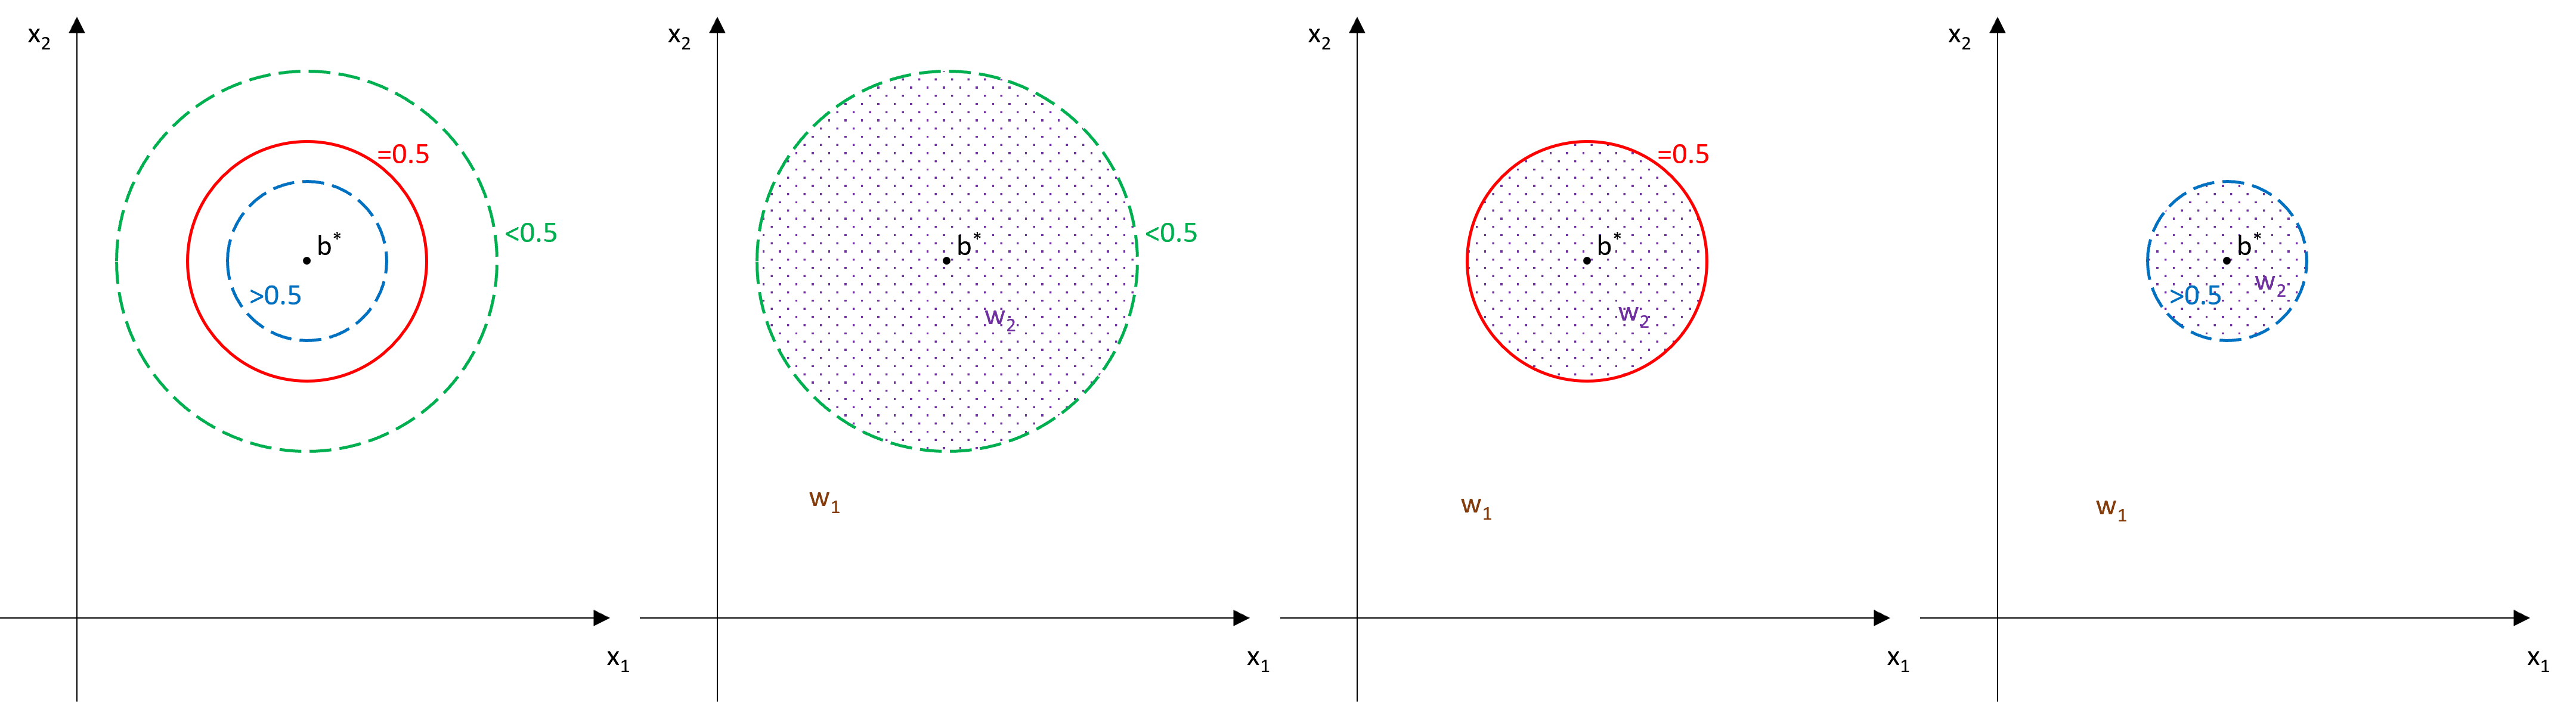
\includegraphics[scale=0.53]{C_4}
    \centering
\end{figure}